\chapter{前提知識}
\label{chap:prerequisite}
本章では,まず深層状態空間モデル(Deep State Space Model, 以下DSSM)のベースとなる変分自己符号化器(Variational Auto Encoder, 以下VAE)について説明し,続いてDSSMの説明を行う.

\section{変分自己符号化器(VAE)}
\label{section:vae}
変分自己符号化器(VAE)は深層生成モデルの一種である.VAEでは,高次元のデータ$\bm{x} \in \mathbb{R}^n$の背後に比較的低次元の潜在表現$\bm{z} \in \mathbb{R}^m$があるとし,Fig. \ref{fig:vae}のようなグラフィカルモデルで表現される確率モデルを考えた上で式(\ref{eq:z})で表されるデータxの確率的生成過程をニューラルネットワークによってモデル化する.

\begin{figure}[tbp]
  \begin{center}
    \begin{tikzpicture}[scale=1, transform shape]
      \node[obs] (x1) {$\bm{x}$};
      \node[latent, above=of x1] (z1) {$\bm{z}$};
      \edge {z1} {x1};
      \end{tikzpicture}
  \caption{VAEのグラフィカルモデル}
  \label{fig:vae}
  \end{center}
  \end{figure}
  
\begin{equation}
  p(\bm{x}) = \int p(\bm{x}|\bm{z}) p(\bm{z}) d\bm{z} \label{eq:vae}
\end{equation}

Fig. \ref{fig:vae}は,高次元なデータ$\bm{x}$は$\bm{x}$の空間上の非常に限られた領域に局所的に存在しているため,それらを低次元の空間で表現可能であるとする多様体仮設に基づいている.また、潜在表現zを考えるると、正しい$P(x|z)$が得られれば,zが与えられたときに$P(x|z)$を使ってそれに対応するxを生成することができ.$P(z|x)$を考えるとxが与えられた際の良い表現としてのzが得られる。

VAEでは,以下の2つの仮定を置き、さらに$p(z|x)$を近似する$q(z|x)$を導入する。$p(x|z)$, $q(z|x)$を適当なニューラルネットワークを使ってモデル化すると,それらのパラメータはデータxが与えられた際に最尤推定によって求めることができる.ただしp(z|x)を直接考えないのは、p(x|z)を表すニューラルネットのパラメータでp(z|x)を表すことが難しいためである..

\begin{eqnarray}
  p(\bm{z}) &=& \mathcal{N}(\bm{z}|0,\bm{I}) \label{eq:z}\\
  p(\bm{z}|\bm{x}) &=& \mathcal{N}(\bm{z}|\mu(\bm{x}),\sigma(\bm{x}))	\label{eq:z_cond}
\end{eqnarray}

式(\ref{eq:z})は,潜在空間が標準正規分布に従っているという仮定であり,式(\ref{eq:z_cond})は,$\bm{x}$に条件づけられた潜在変数の分布が正規分布に従うという仮定である.
$q(z|x)$は推論分布/推論モデルと呼ばれ、グラフィカルモデル中に記述するとFig. \ref{fig:vae_cond}となる.

式(\ref{eq:z})の対数尤度をとることで、以下の変分下限を導出する、

\begin{eqnarray}
  \log p(\bm{x}) &=& \log \int p(\bm{x}|\bm{z}) p(\bm{z}) d\bm{z} \nonumber \\
  &=& \log \int q(\bm{z}|\bm{x}) \frac{p(\bm{x}|\bm{z}) p(\bm{z})}{q(\bm{z}|\bm{x})} d\bm{z} \nonumber \\
  &\geq& \int q(\bm{z}|\bm{x}) \log \frac{p(\bm{x}|\bm{z}) p(\bm{z})}{q(\bm{z}|\bm{x})} d\bm{z} \label{eq:jensen}\\
  &=& \int q(\bm{z}|\bm{x}) \log p(\bm{x}|\bm{z}) d\bm{z} - \int q(\bm{z}|\bm{x}) \log \frac{q(\bm{z}|\bm{x})}{p(\bm{z})} d\bm{z} \nonumber \\
  &=& \mathbb{E}_{\bm{z} \sim q(\bm{z}|\bm{x})} [\log p(\bm{x}|\bm{z})] - \mathrm{D_{KL}}(q(\bm{z}|\bm{x}) \| p(\bm{z})) \label{eq:elbo}
\end{eqnarray}

% \caption[hoge]{fuga}
\begin{figure}[bp]
  \begin{center}
    \begin{tikzpicture}[scale=1, transform shape]
      \node[obs] (x1) {$\bm{x}$};
      \node[latent, above=of x1] (z1) {$\bm{z}$};
      \draw (x1) edge[out=135,in=225,->,dashed] (z1);
      \edge {z1} {x1};
    \end{tikzpicture}
    \caption{推論分布を導入したVAEのグラフィカルモデル.実線は生成分布,点線は推論分布を表す.}
    \label{fig:vae_cond}
  \end{center}
\end{figure}

ここでにはイェンセンの不等式を用いる。
また、数値計算をする都合上式のzの周辺化は難しいため、天下り的に$q(z|x)$を導入する.
式では、zの周辺化を解析的には計算できないため,$q(z|x; \phi)$からサンプリングされる$L$個の$\bm{z}$を用いて$\frac{1}{L} \sum_{l} \log p(\bm{x}|\bm{z})$でモンテカルロ近似する.
ただし通常L=1で計算される。
またこの近似は、式でp(z)からzをサンプリングすることと比較して現実的な計算コストに抑えられるに注意されたい。
式(\ref{eq:elbo})の第2項の$\mathrm{D_{KL}}$(カルバックライブラー距離)は,いま$p(\bm{z})$,$q(\bm{z}|\bm{x}; \phi)$共にガウス分布を仮定しているため,解析的に計算することができる.
式(\ref{eq:elbo})の第1項は、p(x|z)の分布に正規分布やベルヌーイ分布を仮定することで二乗誤差やクロスエントロピー誤差として計算できる。

この変分下限を目的関数にしてNNを学習させる.
以上がVAEの概要である.このように学習されたVAEは,事前分布$p(\bm{z})$から$\bm{z}$をサンプリングし,デコーダを通すことでFig. \ref{fig:vae_example}のような新たなデータを生成することができる.左は顔画像のデータセットFrey Faceを用いて学習したVAEによって生成された画像,右はMNISTで学習したVAEの生成画像である.

% \caption[hoge]{fuga}
\begin{figure}[tbp]
  \begin{center}
    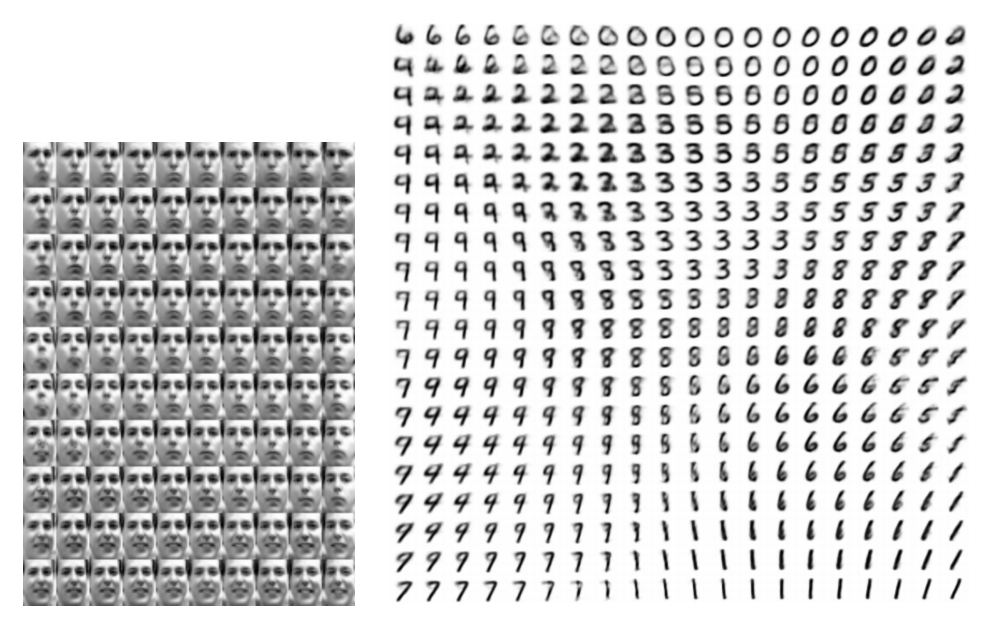
\includegraphics[width=\linewidth]{./figures/vae.png}
    \caption{VAEを用いて生成された画像の例(\cite{vae}より引用)}
    \label{fig:vae_example}
  \end{center}
\end{figure}

\section{深層状態空間モデル(DSSM)}
\label{section:dssm}

深層状態空間モデル(DSSM, Deep Karman Filters, Deep Markov Modelなどとも呼ばれる)は、VAEがデータ一つ一つの潜在表現を考えるのに対し、DSSMは時間変化があるデータの各時刻の状態表現が遷移すると考えたモデルであり、VAEを時系列方向に拡張したモデルとみなすこともできる.

深層強化学習の分野では、エージェントが環境に行動を起こした結果に観測が得られるようなときに、行動と環境の変化をモデル化する際に用いられる.本論文では一般的な以下のようなグラフィカルモデルで表されるDSSMのモデルを考えるが、行動が与えられない場合や、強化学習のように環境の状態に応じて報酬が与えられる問題に置いても以下の説明は同様にして考えることができる
.
DSSMではVAEと同じように,以下の変分下限から最尤推定によって$p(o|a)$や$p(s|x)$を得る.

\begin{eqnarray}
  \log p(o_{1:T}|a_{1:T})
  &=& \log \prod_{t=1}^T p(o_t|a_{1:t}) \nonumber \\
  &=& \log \prod_{t=1}^T \int p(o_t|s_t) p(s_t|s_{t-1}, a_t)ds_t \nonumber \\
  &=& \sum_{t=1}^T \log \int p(o_t|s_t) p(s_t|s_{t-1}, a_t)ds_t \nonumber \\
  &=& \sum_{t=1}^T \log \int q(s_t|s_{t-1}, a_t, o_t) \frac{p(o_t|s_t) p(s_t|s_{t-1}, a_t)}{q(s_t|s_{t-1}, a_t, o_t)}ds_t \nonumber \\
  &\geq& \sum_{t=1}^T \int q(s_t|s_{t-1}, a_t, o_t) \log \frac{p(o_t|s_t) p(s_t|s_{t-1}, a_t)}{q(s_t|s_{t-1}, a_t, o_t)}ds_t \nonumber \\
  &=& \sum_{t=1}^T \left( \int q(s_t|s_{t-1}, a_t, o_t) \log p(o_t|s_t)ds_t \right. \nonumber \\
  && \hspace{2em} \left. - \int q(s_t|s_{t-1}, a_t, o_t) \log \frac{p(s_t|s_{t-1}, a_t)}{q(s_t|s_{t-1}, a_t, o_t)}ds_t \right) \nonumber \\
  &=& \sum_{t=1}^T \left( \mathbb{E}_{s_t \sim q(s_t|s_{t-1}, a_t, o_t)} [\log p(o_t|s_t)] \right. \nonumber \\
  && \hspace{2em} \left. - \mathbb{E}_{s_{t-1} \sim q(s_{t-1}|s_{t-2}, a_{t-1}, o_{t-1})} [\mathrm{D_{KL}}(q(s_t|s_{t-1}, a_t, o_t) \| p(s_t|s_{t-1}, a_t, o_t))] \right)  \nonumber \\
  \label{eq:dssm_elbo}
\end{eqnarray}

ただし$s_0$は、初期状態が一定な問題を考える際は常にゼロベクトルなど一定の値にすることもあるが,そうでない場合は何らかの方法で推論する必要がある.本研究では慣例に習って$s_0$を$s_0 \sim q(s_0|\vec{0}, \vec{0}, o_0) $によって定め,(\ref{eq:dssm_elbo})の第2項の$s_0$のサンプリングはこれで置き換える.

式は、イェンセンの不等式を使い、qはpの近似である.

以上がDSSMの概要である.DSSMを用いると, \ref{fig:dssm_planet}, \ref{fig:dssm_dkf}のような新たなデータを生成することができる.actionとして回転情報が入れられている.

\begin{figure}[tbp]
  \begin{center}
    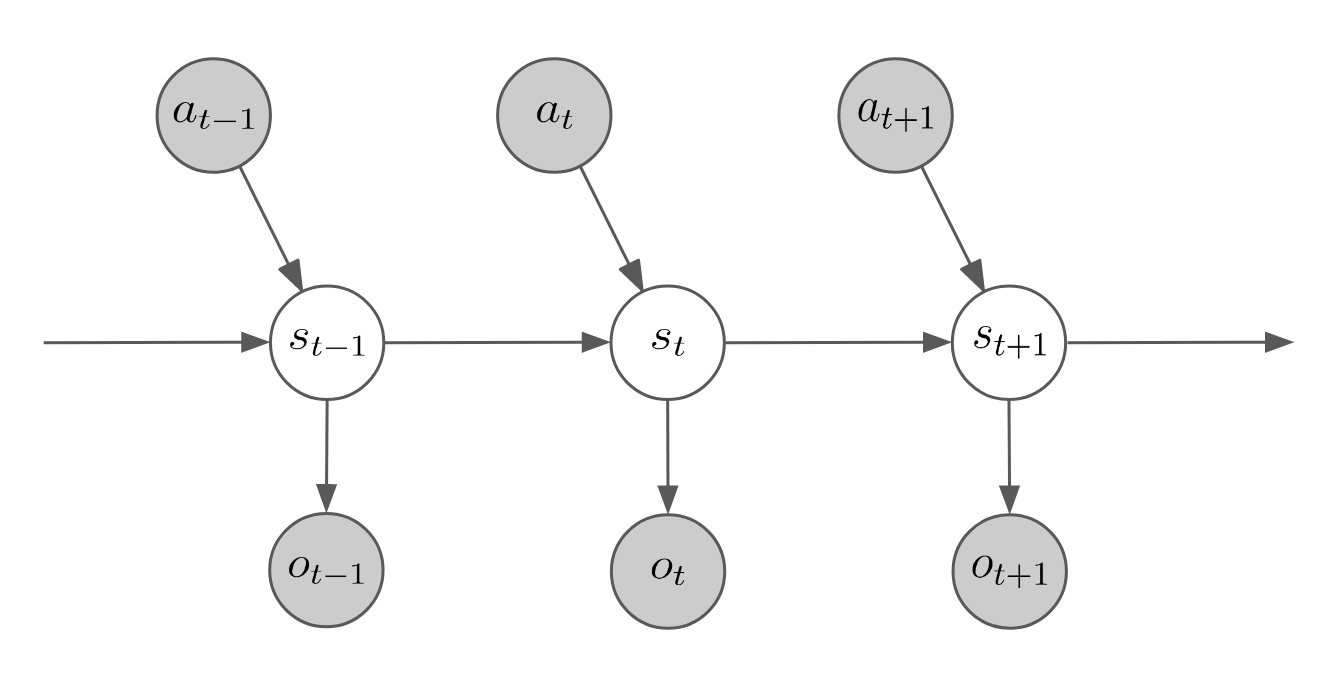
\includegraphics[width=\linewidth]{./figures/dssm.png}
    \caption{SSMのグラフィカルモデル}
    \label{fig:ssm}
  \end{center}
\end{figure}

% \caption[hoge]{fuga}
\begin{figure}[tbp]
  \begin{center}
    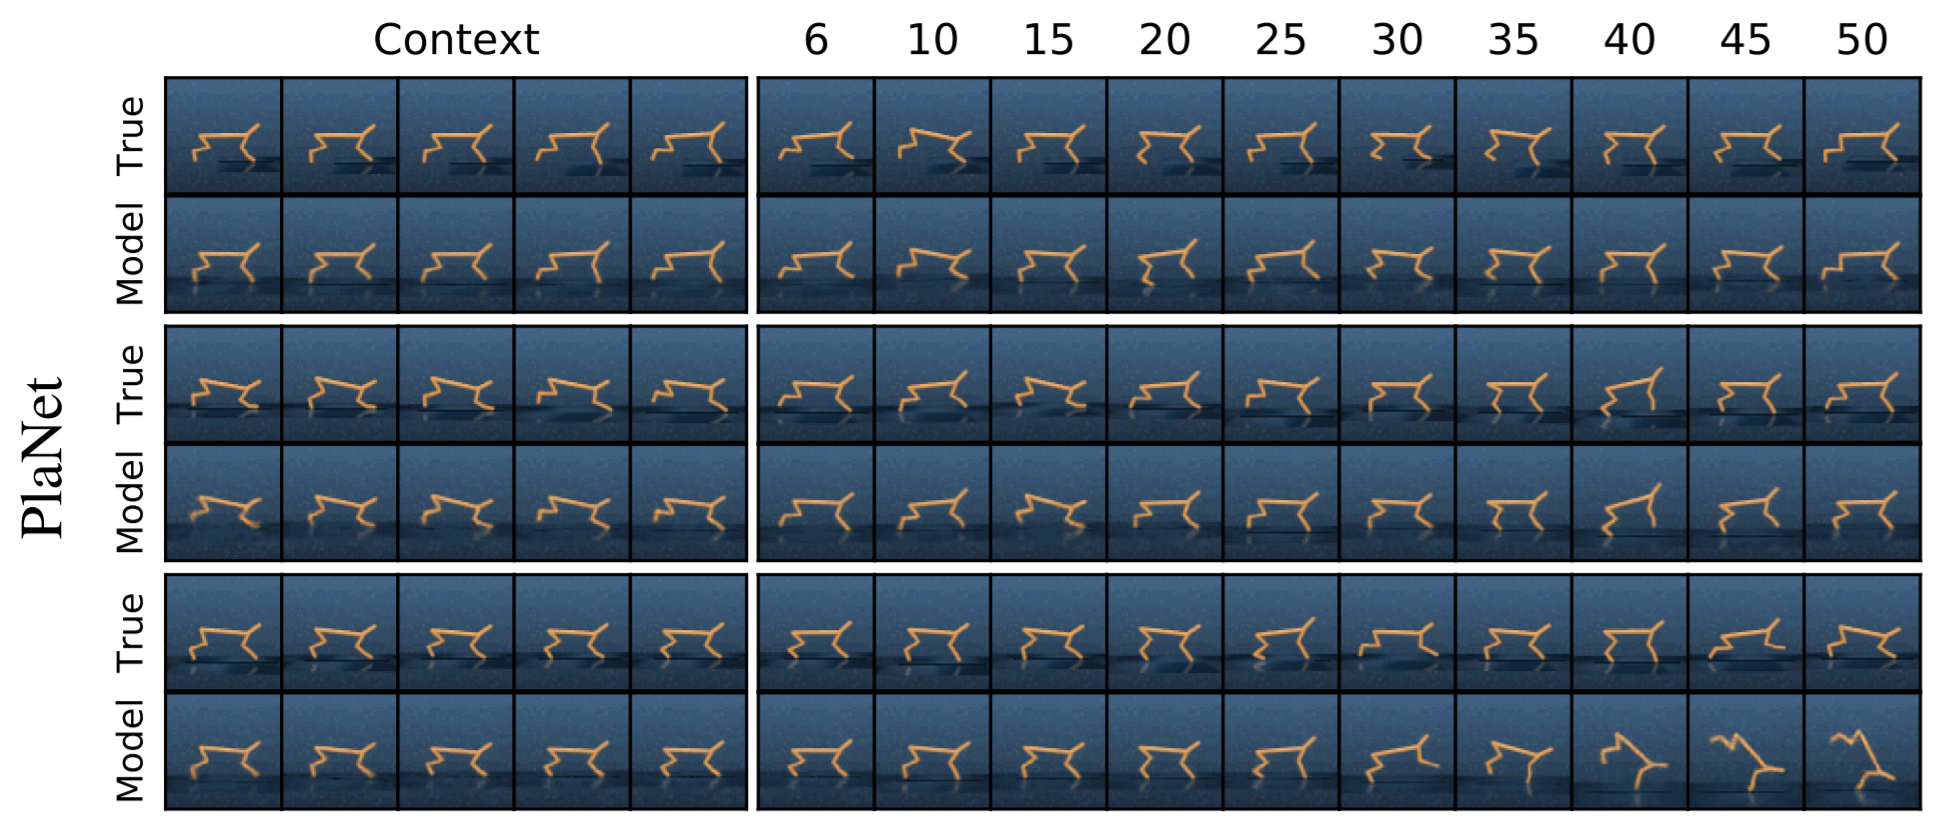
\includegraphics[width=\linewidth]{./figures/dssm_planet.png}
    \caption{DSSMで生成される映像の例.ただしSSMを少し拡張したRSSMモデルを使っている}
    \label{fig:dssm_planet}
  \end{center}
\end{figure}

% \caption[hoge]{fuga}
\begin{figure}[tbp]
  \begin{center}
    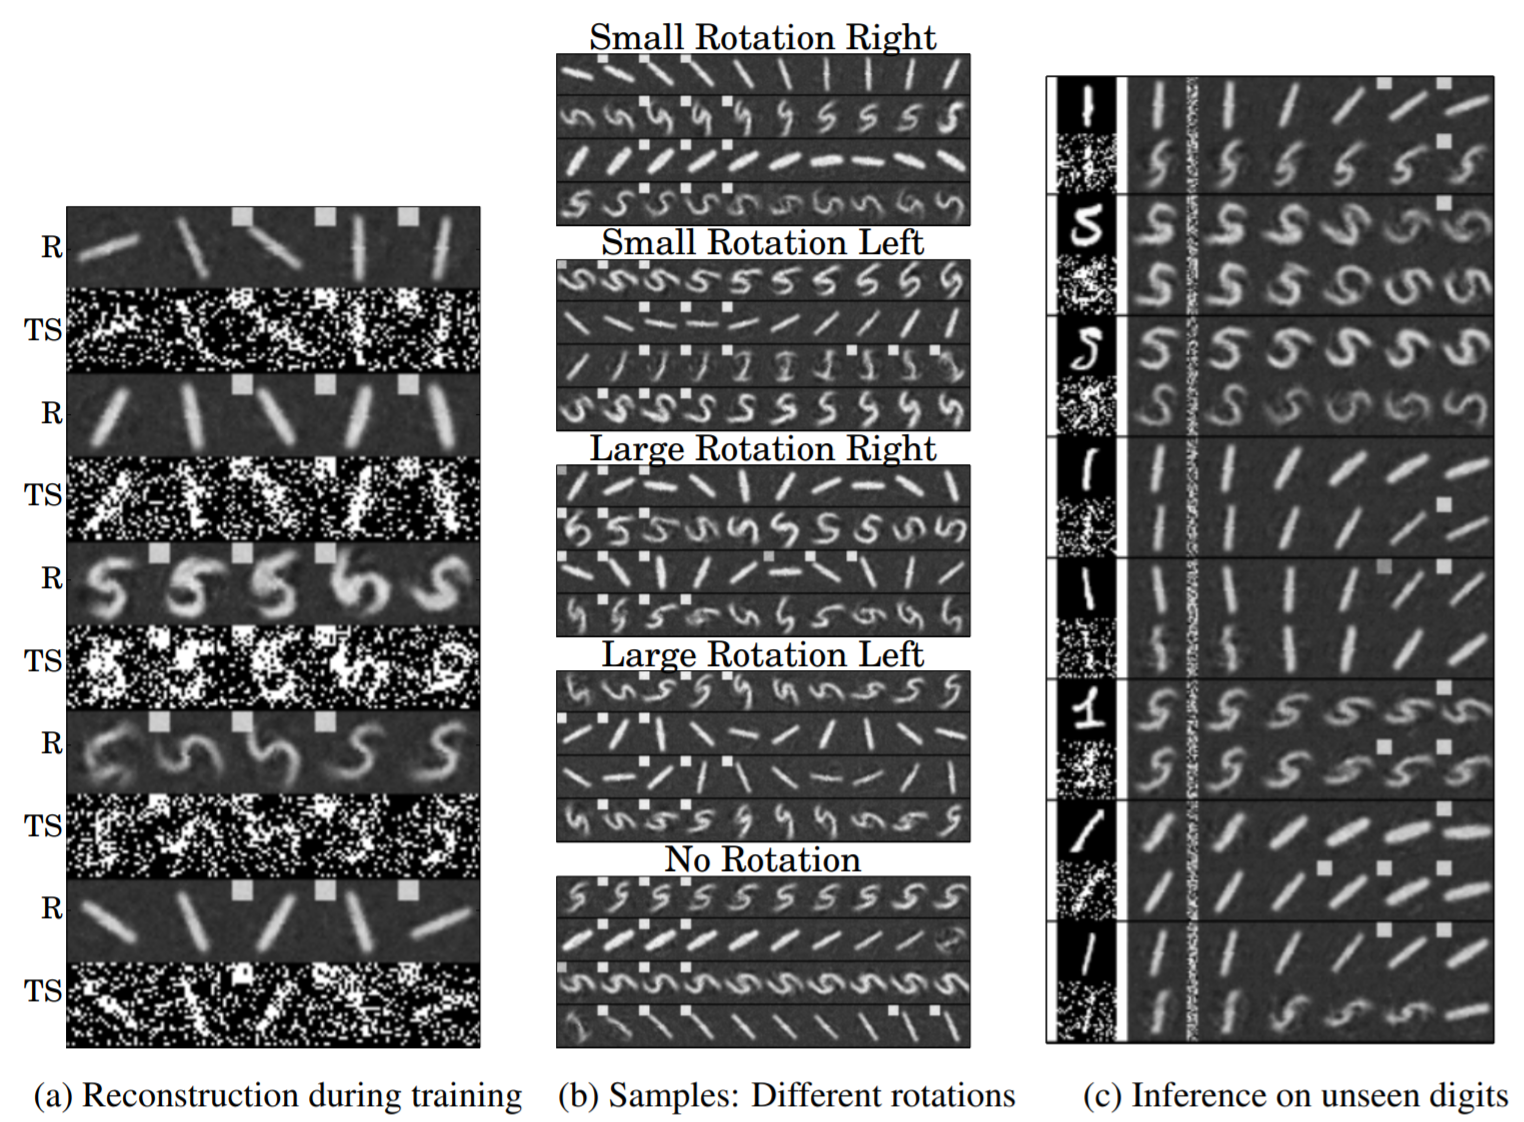
\includegraphics[width=\linewidth]{./figures/dssm_dkf.png}
    \caption{DSSMで生成される映像の例.}
    \label{fig:dssm_dkf}
  \end{center}
\end{figure}